\chapter{Representación.}\label{cap:capitulo3}

Entraremos en detalle de la representación de los distintos elementos que componen el generador. Repasaremos el concepto de \emph{mapa de tiles} de nuevo. Analizaremos la representación lógica y física necesaria con el objetivo de establecer un modelo claro para las habitaciones y el mapa que usaremos posteriormente para la construcción del sistema de generación.


En nuestro contexto, disponemos de tres tipos de entidades:

\begin{itemize}
	\item \emph{Habitaciones} que compondrán el mapa.
	\item \emph{Mapa} o escenario donde se desarrolla el juego, compuesto por habitaciones. Posee algunos elementos ausentes en las habitaciones.
	\item \emph{Puertas} que servirán de conexión entre habitaciones.
\end{itemize}

Es importante tener claro el aspecto de la representación de las entidades que se utilizarán en el sistema, ya que el mismo se construirá en base a lo que se detalle en la representación.

\section{Topología.}

Como se ha repetido varias veces anteriormente, usaremos un \emph{mapa de tiles} para la representación del escenario. Esto implica que los modelos tanto de las habitaciones como del propio mapa, han de mantener una matriz para la representación física. En la figura~~\ref{fig:memtiles} podemos ver la representación en memoria como una matriz de un mapa de tiles. En la figura~\ref{fig:graftiles} se observa la representación gráfica. Se puede comprobar la relación directa entre ambas representaciones.


\begin{figure}[h]
\centering
{
	$
\begin{matrix}
	0 & 1 & 1 & 1 & 0 \\
	0 & 1 & 0 & 1 & 1 \\
	1 & 1 & 0 & 0 & 1 \\
	1 & 0 & 0 & 0 & 1 \\
	1 & 1 & 1 & 1 & 1
\end{matrix}
$
}
\caption{Representación en memoria de un mapa de tiles
\label{fig:memtiles}
}
\end{figure}

\begin{figure}[t]
\centering
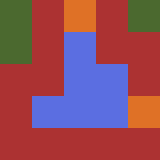
\includegraphics[scale=1]{img/graftiles}
\caption{Representación gráfica de un mapa de tiles
\label{fig:graftiles}}
\end{figure}

En principio, los tipos de tile que se han considerado son los siguientes:

\begin{itemize}
	\item \textcolor{red}{\emph{Tile pared}}. Representa una porción de geometría sólida infranqueable. A la hora de colocar habitaciones, habrá que añadir un mecanismo para evitar el solapamiento entre tiles sólidos de entidades distintas.
	\item \textcolor{blue}{\emph{Tile interior}}. Representa una porción de geometría traspasable. A igual que el tile sólido, habrá que evitar solapamiento con tiles pertenecientes a otras entidades (habitaciones o el mapa).
	\item \textcolor{OliveGreen}{\emph{Tile exterior}}. Representa una porción de geometría traspasable \emph{externa} a la habitación. Este tipo de tiles sí que puede solaparse con tiles pertenecientes a otras entidades.
	\item \textcolor{orange}{\emph{Tile puerta}}. Representa una conexión entre dos habitaciones. No podrá solaparse, pero si traspasarse para permitir el cruce entre habitaciones.
\end{itemize}

En la figura~~\ref{fig:proptiles} se ve un resumen de las propiedades inherentes a cada tipo de tile.

\begin{figure}[h]
\centering
{
\begin{tabular}{|c|c|c|}
\hline
		& Sólido 		& Solapable 	\\
\hline
Pared 	&  \checkmark  	&  X  			\\ \hline
Interno &  X			&  X  			\\ \hline
Externo &  X  			&  \checkmark  	\\ \hline
Puerta  &  X  			&  X 		 	\\ \hline
\end{tabular}
}
\caption{Propiedades de los tiles
\label{fig:proptiles}
}

\end{figure}



Con todo ésto, ya tenemos clara la representación física de los distintos elementos implicados en el sistema de generación. Ahora, entraremos en detalle con elementos específicos para el mapa y la habitación, que principalmente nos serán necesarios para algunas optimizaciones y llevar a cabo la lógica del generador.

Más adelante veremos un tipo de tile especial (tile tipo \emph{puerta}) en el que nos apoyaremos para la conexión entre habitaciones.

\section{Habitaciones.}

Analizaremos los elementos relevantes para la representación de las habitaciones. Atendiendo a la especificación de que las habitaciones \emph{se pueden repetir}, se ha dividido la representación en dos componentes:

\begin{itemize}
	\item \emph{Prefab}. Representación que engloba los elementos comunes para un modelo de habitación. Sirve, entre otras cosas, para almacenar solamente un mapa de tiles por modelo de habitación.
	\item \emph{Instancia}. Representación específica para una concretización o instancia de un modelo de habitación o prefab. Contendrá información sobre la posición de una habitación en el mapa y las puertas.
\end{itemize}

Ésto nos permite un ahorro de memoria, ya que guardamos información común a muchas habitaciones en un solo modelo, y procesamiento, que veremos en detalle en el capítulo ~\ref{cap:capitulo4}.

\subsection{Puertas potenciales.}

Antes de abarcar los dos componentes empleados para representar las habitaciones, vamos a introducir el concepto de \emph{puerta potencial}, que será necesario para explicar una de las motivaciones del \emph{prefab}, además de tener que mantener solo un mapa de tiles por modelo.

Con el concepto de puertas potenciales nos referimos a las posibles conexiones de un modelo de habitación. Cualquier tile que cumpla la restricción de ser puerta potencial, puede convertirse en puerta para establecer una conexión entre habitaciones en el transcurso de la generación en el sistema.

Así, consideraremos que un tile $t(x,y)$ será una puerta potencial de la habitación $R$ teniendo en cuenta las dos orientaciones posibles. 

\begin{itemize}
	\item \textcolor{blue}{\emph{Horizontal}} si se cumple:
	\begin{itemize}
		\item Existe un tile \emph{pared} a la izquierda y derecha del tile.
		\item Existe un tile \emph{interior} arriba y un tile \emph{exterior} abajo, o viceversa.
	\end{itemize}
	\item \textcolor{red}{\emph{Vertical}} si se cumple:
	\begin{itemize}
		\item Existe un tile \emph{pared} arriba y abajo del tile.
		\item Existe un tile \emph{interior} a la izquierda y un tile \emph{exterior} a la derecha, o viceversa.
	\end{itemize}
\end{itemize}

\begin{figure}[t]
\centering
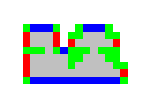
\includegraphics[scale=1]{img/ppot}
\caption{Representación gráfica de puertas potenciales \textcolor{red}{verticales} y \textcolor{blue}{horizontales}
\label{fig:grafpp}}
\end{figure}

En la figura~\ref{fig:formpp} se puede ver la definición formal del concepto de \emph{puerta potencial}, y en la figura~\ref{fig:grafpp}, una representación gráfica, teniendo en cuenta ambos casos.

\begin{figure}[h]
\centering
{
$$
t \in R, \begin{cases}
	outer(x+1,y), \quad inner(x-1,y), \quad wall(x, y\pm1) & \quad vertical \\
	outer(x-1,y), \quad inner(x+1,y), \quad wall(x, y\pm1) & \quad vertical\\
	outer(x,y+1), \quad inner(x,y-1), \quad wall(x\pm1, y) & \quad horizontal\\
	outer(x,y-1), \quad inner(x,y+1), \quad wall(x\pm1, y) & \quad horizontal\\
\end{cases}
$$

}
\caption{Definición formal de una puerta potencial y sus casos
\label{fig:formpp}
}
\end{figure}

Según la complejidad de las habitaciones, con este concepto conseguiremos ahorrarnos casos en los que será imposible conectar habitaciones. Obviamente, habrá casos en los que aún siendo un tile una puerta potencial, es imposible conectarla con otra habitación por motivos de solapamiento entre las mismas. Aún así, podemos ahorrarnos parte de las comprobaciones.

\subsection{Prefabs.}

Como se ha mencionado anteriormente, los prefabs representarán el modelo de un tipo de habitación, común a todas las instancias o concretizaciones del mismo. Las motivaciones de este componente son de eficiencia, tanto de memoria como de procesamiento.

En cuanto a memoria, solo tendremos que guardar un mapa de tiles, ya que las instancias correspondientes a un prefab, guardarán la misma representación física. Además, solo será necesario guardar la lista de puertas potenciales en el prefab, ya que también será común a todas las instancias.

El cómputo de las puertas potenciales también conlleva un coste, y gracias a este componente, se realizará una sola vez en la carga.

\subsection{Instancias.}

La instancia representa una concretización de un prefab. Una vez tenemos los modelos de habitación necesarios, se crearán las instancias pertinentes a partir de cada modelo. En estas instancias, incluiremos la información necesaria para situar las habitaciones en el mapa, así como para poder manejar las conexiones entre puertas de las distintas instancias de habitaciones y poder realizar estimaciones sobre el mapa.

Para conectar dos instancias de habitación, necesitaremos una puerta por cada instancia, de forma que ambas puertas sean contiguas para que el jugador pueda cruzar de una habitación a otra. En la figura~\ref{fig:instp} se puede observar la definición formal de ésto.

\begin{figure}[h]
\centering
{
$$
p1(x1,y1) \in R1, p2(x2,y2) \in R2, \begin{cases}
	p1 = p2 + (0,1) & \quad \text{conexión horizontal} \\
	p1 = p2 - (0,1) & \quad \text{conexión horizontal} \\
	p1 = p2 + (1,0) & \quad \text{conexión vertical}   \\
	p1 = p2 - (1,0) & \quad \text{conexión vertical}   \\
\end{cases}
$$
}
\caption{Conexión entre dos instancias de habitación
\label{fig:instp}
}
\end{figure}

Así, guardaremos una lista de las puertas presentes en la instancia.

Otro dato importante a mantener en a instancia es una referencia al prefab, de forma que podamos realizar los cómputos necesarios que corresponden al modelo de habitación.

Por último, necesitaremos conocer la posición de la instancia en el mapa. Esta posición no se usará mientras la instancia no esté colocada en el mapa. Asimismo, se establecerá el valor de este dato, cuando coloquemos la instancia en el mapa.

Cabe destacar que a efectos lógicos, dos instancias de un mismo prefab son consideradas como habitaciones \emph{distintas}. La utilización del prefab es solo una medida de conveniencia para evitar la duplicación de información.

\section{Puertas.}

Una vez elegido un par de tiles de puertas potenciales de dos instancias de habitación distintas que conectaremos, tenemos que añadir cierta información a las puertas, que será necesaria para el funcionamiento del sistema.

\begin{itemize}
	\item \emph{Instancia de Habitación propietaria} de la puerta
	\item \emph{Puerta conectada} miembro de la instancia de habitación conectada.
	\item La \emph{habitación conectada} se puede extraer a partir de la \emph{puerta conectada}.
	\item \emph{Posición local} relativa a la instancia de habitación a la que pertenece la puerta.
	\item \emph{Tipo} de puerta. Se refiere a la orientación: horizontal o vertical.
\end{itemize}

Con toda esta información, podemos tratar las puertas como elementos independientes, ya que se tiene acceso a todos los componentes necesarios para cualquier cómputo o acción que desee realizarse sobre la conexión que representa esta puerta.

\section{Mapa.}

Por último, el modelo que usaremos para el mapa contendrá información física y lógica de las habitaciones y su disposición en el escenario.

El modelo empleado para el mapa, empleará un mapa de tiles donde se colocarán las habitaciones de forma física. El mapa de tiles nos servirá para comprobar solapamiento a la hora de colocar habitaciones para conectarlas. Además, una vez completo el mapa, tendremos el resultado final de la generación en este mapa de tiles. 

El mapa de tiles empleado en el mapa, según las especificaciones, se supone lo suficientemente grande como para albergar cualquier distribución de habitaciones. Se ha elegido hacer uso de un mapa de tiles lo suficientemente grande para cumplir este requisito, pero podría haberse elaborado un mapa autoajustable, de forma que, en caso de ser necesario, se expandiría el tamaño.

Resultará práctico mantener las conexiones entre las instancias de habitaciones presentes en el mapa. Para ello, se ha hecho uso de una matriz superior, tal que en cada posición $(R1,R2)$, tendremos una estimación de la distancia entre las habitaciones $R1$ y $R2$. Consideraremos un valor muy alto como la ausencia de conexión. Esta matriz superior nos será de mucha utilidad a la hora de computar propiedades del mapa de forma rápida.

También será útil mantener una lista con el conjunto de todas las puertas potenciales de las habitaciones en el mapa. Se hablará en detalle de ésto en el próximo capítulo.
